\section{Aproximação de curta distância}
\label{sec_fases_app_curta}

Na fase de aproximação de curta distância, o movimento relativo entre as espaçonaves passa a ser descrito no referencial \gls{lvlh} centrado no alvo. 
Nesse regime, a dinâmica relativa é modelada por meio das equações linearizadas de \gls{hcw}, que descrevem a evolução da posição e da velocidade relativas do perseguidor em relação ao alvo.

Para conduzir o perseguidor até a posição desejada, emprega-se uma lei de controle \gls{pd} aplicada ao movimento translacional relativo. 
Esse controlador atua sobre o erro entre a posição relativa atual e a posição de referência, gerando as acelerações de controle necessárias para reduzir o erro de trajetória e garantir uma aproximação suave.

Devido à maior proximidade entre as espaçonaves, torna-se também possível estimar a atitude do alvo por meio dos sensores do perseguidor. 
A orientação medida do alvo é então comparada com a atitude do perseguidor, permitindo aplicar uma segunda lei de controle \gls{pd} responsável pelo alinhamento de atitude entre as duas espaçonaves.
A Figura~\ref{fig_fluxo_app_curta_distancia} apresenta o fluxograma da estratégia de controle empregada nessa fase, indicando a interação entre o modelo de dinâmica relativa, o cálculo do erro de posição e velocidade e a geração das acelerações de controle.

\begin{figure}[H]
\centering
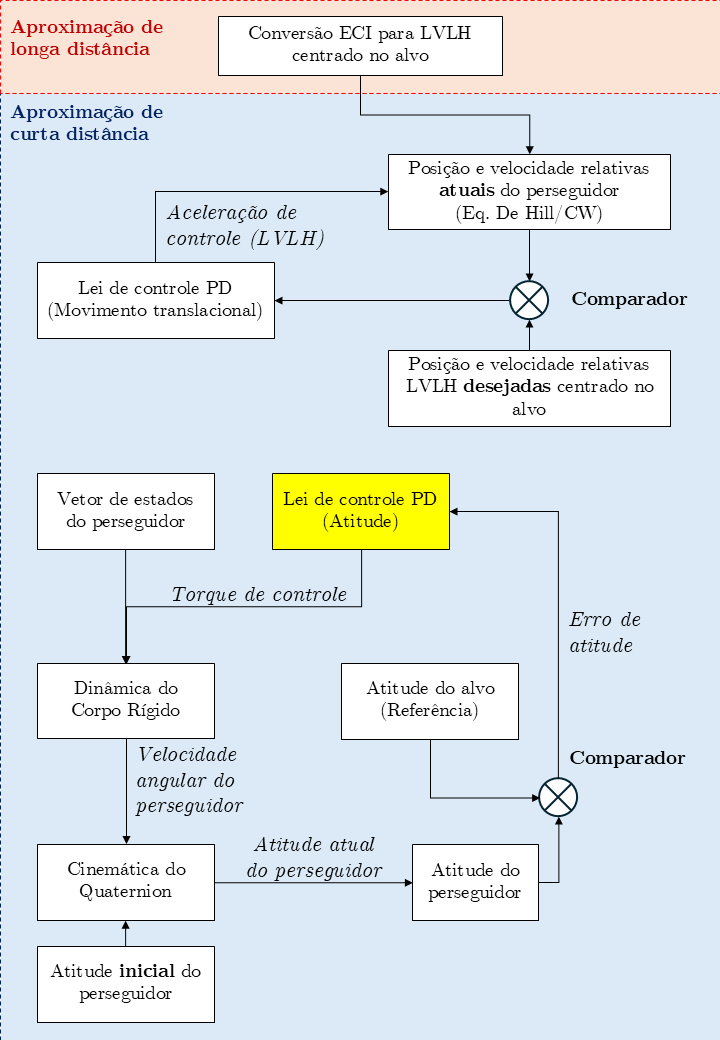
\includegraphics[width=1\linewidth]{3 Procedimento simulacao/Imagens diagrama/3 App curta.png}
\caption{Fluxo da aproximação de curta distância.}
\label{fig_fluxo_app_curta_distancia}
\end{figure}

A implementação da dinâmica relativa baseada nas equações de \gls{hcw} foi realizada no ambiente Simulink por meio de uma representação em espaço de estados, conforme ilustrado na Figura~\ref{fig_hcw_space_state}. 
Nessa estrutura, as equações diferenciais que descrevem o movimento relativo são organizadas em um subsistema responsável pela propagação da posição e da velocidade relativas.

\begin{figure}[H]
\centering

\includegraphics[width=1\linewidth]{3 Procedimento simulacao/Imagens simulink/app_curta_hcw_space_state.png}
\caption{Implementação das equações de \gls{hcw} em espaço de estados no ambiente Simulink.}
\label{fig_hcw_space_state}
\end{figure}
O controlador \gls{pd} responsável pela geração das acelerações de controle foi implementado de forma independente para cada eixo do referencial \gls{lvlh}. 
A Figura~\ref{fig_controle_pd_radial} apresenta a estrutura utilizada para o eixo radial, sendo a mesma lógica aplicada aos eixos along-track e cross-track.


\begin{figure}[H]
\centering

\includegraphics[width=1\linewidth]{3 Procedimento simulacao/Imagens simulink/app_curta_controle_pd_radial.png}
\caption{Implementação da lei de controle \gls{pd} para o movimento relativo no eixo radial.}
\label{fig_controle_pd_radial}
\end{figure}

Durante a aproximação de curta distância, também é aplicada uma lógica de limitação de velocidade relativa, conforme proposto por \cite{vedant2025longrange}, com o objetivo de garantir segurança durante a manobra. 
Para distâncias superiores a $20$~m do alvo, o limite de velocidade é definido como $0,300$~m/s. 
Quando o perseguidor se encontra a menos de $20$~m do alvo, esse limite é reduzido para $0,030$~m/s, permitindo maior precisão durante a fase final da aproximação.

Além do critério baseado na distância, foi introduzida uma janela temporal de $15$~s para validar a transição entre os regimes de limitação de velocidade. 
Dessa forma, o perseguidor deve permanecer continuamente dentro ou fora do limite de $20$~m durante esse intervalo de tempo para que a troca de limite seja efetivada. 
Essa estratégia foi adotada para evitar comutações rápidas entre os dois limites de velocidade, que poderiam gerar oscilações no sistema de controle e comprometer a estabilidade da manobra, o bloco relacionado é apresentado na Figura~\ref{fig_limite_velocidade}.

\begin{figure}[H]
\centering
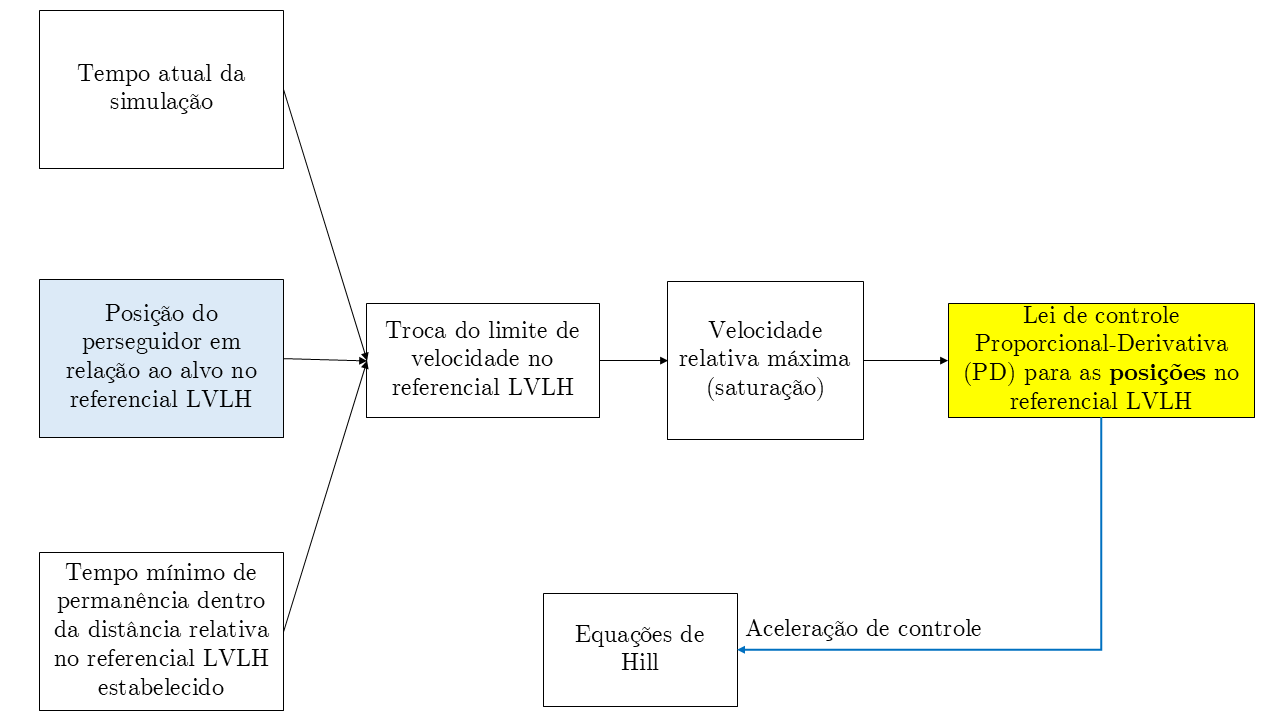
\includegraphics[width=1\linewidth]{3 Procedimento simulacao/Imagens simulink/app_curta_limite_velocidade.png}
\caption{Implementação da lógica de limitação de velocidade relativa durante a aproximação.}
\label{fig_limite_velocidade}
\end{figure}

Por fim, como apresentado na Figura~\ref{fig_tempo_estabilizacao}, foi implementado um subsistema dedicado à avaliação do desempenho do controlador, responsável pela medição do tempo necessário para estabilização da posição relativa no eixo radial. 
A mesma lógica é aplicada aos eixos along-track e cross-track.

\begin{figure}[H]
\centering

\includegraphics[width=1\linewidth]{3 Procedimento simulacao/Imagens simulink/app_curta_tempo_estabilizacao.png}
\caption{Estrutura utilizada para medição do tempo de estabilização da posição relativa.}
\label{fig_tempo_estabilizacao}
\end{figure}